\section{Resultado}

O algoritmo foi testado com $\alpha = 4200$ e precisão de inteiro,
o que resultou na seguinte waveform.

    \begin{figure} [H] 
        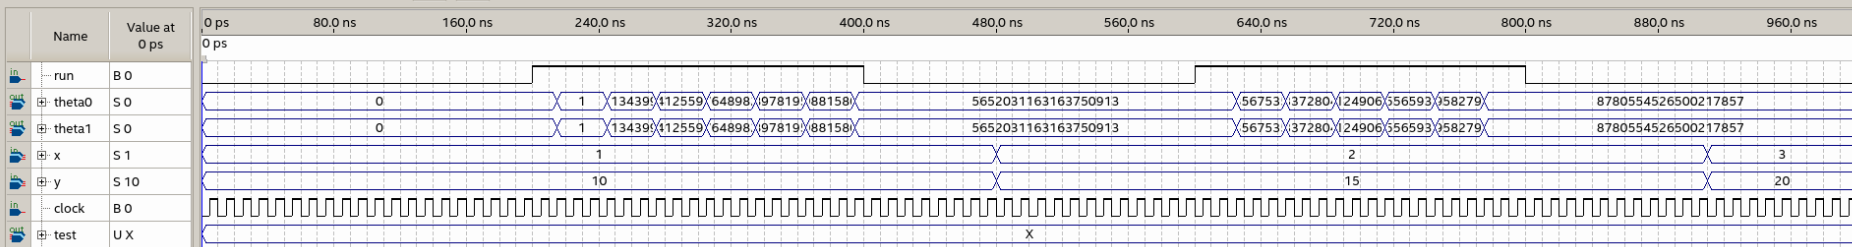
\includegraphics[width=\textwidth]{waveform}
        \caption{Waveform - baixa precisão}
        \label{fig:waveform}
    \end{figure}

Que nunca se aproxima do valor correto por sua baixa precisão e alta taxa de atualização.

    \begin{figure} [H] 
        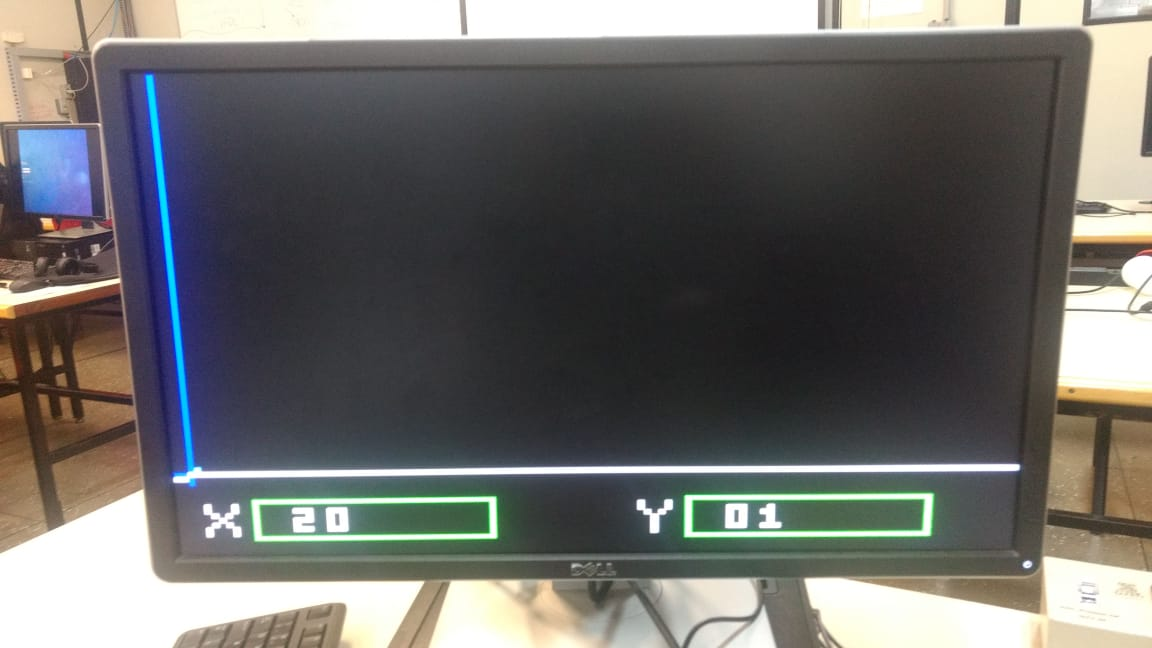
\includegraphics[width=\textwidth]{monitor}
        \caption{Monitor}
        \label{fig:monitor}
    \end{figure}

    \begin{figure} [H] 
        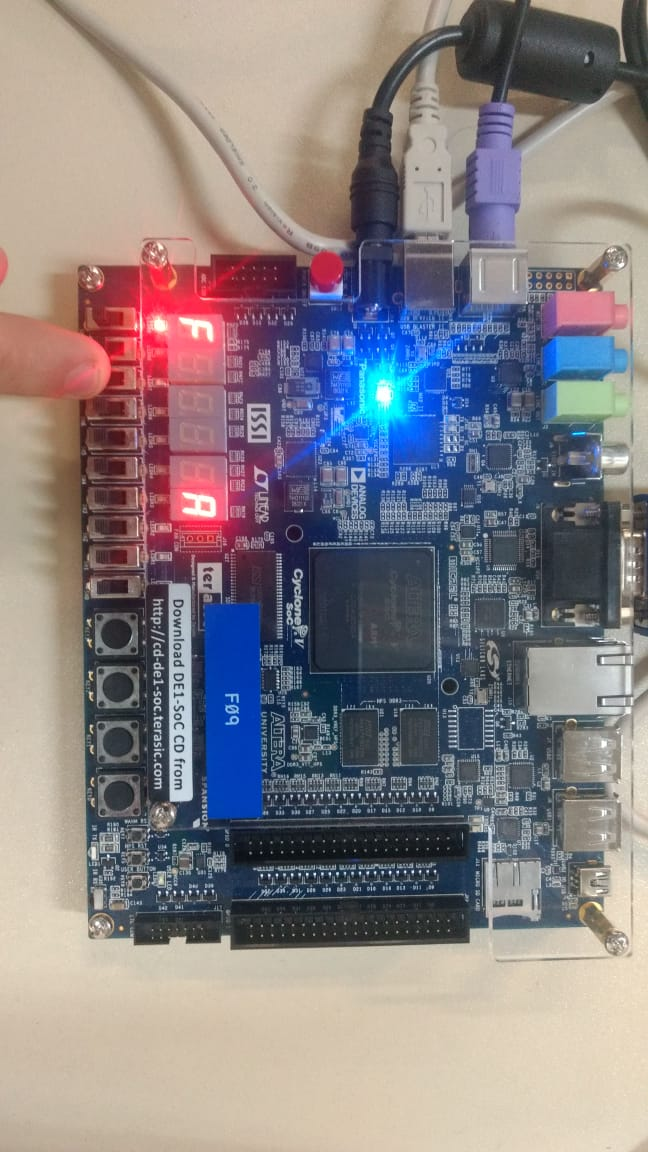
\includegraphics[width=\textwidth]{fpga}
        \caption{FPGA}
        \label{fig:fpga}
    \end{figure}

Então foi testado no monitor, com precisão de ponto fixo de 32 casas.
Mas a precisão fez com que todos os valores virassem 0

\subsection{O que faltou}

O algoritmo, embora pronto, ainda não foi completamente implementado no montitor.

Os seguintes bugs foram encontrados:

\begin{itemize}
    \item Limpar a tela, não funciona
    \item Desenho do gráfico sai dos limites
\end{itemize}

Os seguintes itens poderiam ainda ser implementados:

\begin{itemize}
    \item Desenhar os pontos do vetor na tela
    \item Função de apagar dígito (Backspace)
    \item Função de mudar de campo (Tab)
    \item Suporte para input de números negativos
    \item Suporte para input de números decimais
    \item Aumentar a resolução
\end{itemize}
